\section{Magnetism}
Up until this point we haven't taken much of a  look at the behavior of charges in motion, or the magnetic field and how it is related to the electric field. The symbol we will use for the magnetic field is $\vec B$ (because apparently, the letter M is just too common), and the magnetic field is measured in units of teslas (T). However, a 1 T magnetic field is really strong (for context, the Earth's magnetic field has a strength of 0.25-0.65 microteslas). We also define the gauss, which is $10^{-4}$ teslas, which we will also use to measure the strength of magnetic fields. We will look at how we can calculate this field, how it arises and interacts with charges, and how a changing magnetic field can actually induce, or create an electric field. 
\subsection{Lorentz Force}
Up until this point, we've only talked about the electric force on a charged particle, where $\vec E = \frac{\vec F}{q}$ or $\vec F = q\vec E$. This is not the full picture - the magnetic field also exerts a force on charged particles, and the full expression for the electromagnetic force on a charged particle (the Lorentz force) is the following:
\[
	\vec F = q\vec E + q\vec v \times \vec B
\]
This second term is the magnetic force on a charged particle, which is dependent on the velocity of the particle. This dependency means that the magnetic force is non-conservative - it cannot have a potential energy function because it is dependent on factors other than the position of the particle. However, the magnetic force also does no work on a charged particle - to see this, notice that the magnetic force always acts perpendicular to the direction that the force is moving, so the dot product, when evaluated, will be zero. This is strange - the magnetic force does not do work on a charged particle but is non-conservative, but that's just how it works. There is such a thing as magnetic (vector and scalar) potential - but there's no need to worry about that.\\
When we deal with magnetic forces, we usually deal with relatively simple cases. The first is the case of a "velocity selector" - the setup is a region where the electric field $\vec E$ and magnetic field $\vec B$ are perpendicular to each other and let's say that a beam launches (positively) charged particles at various velocities through this region. What velocity-particles will not be deflected by the electromagnetic field? \\
\begin{center}
	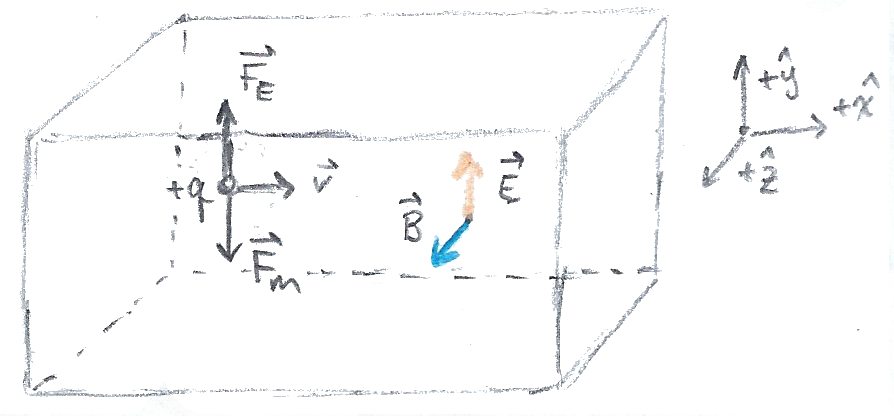
\includegraphics[width=0.5\textwidth]{images/em/velocity-selector.png}
\end{center}
To find this out, we can assume that the velocity is in the $+x$-direction, the electric field is in the $+y$-direction, and the magnetic field is in the $+z$-direction. In order for the motion of the particle to remain unchanged, the force must be zero. \\
Before we do any calculations, let's figure out if this is possible by checking the directions of the two forces. The electric force must be in the $+y$-direction, as the electric field and the electric force are proportional, and the magnetic force must be in the direction that $\hat x \times \hat z$ points in. Using the right-hand rule, this points in the $-y$-direction, so we're sure that this is possible. (If they didn't point in opposite directions, we'd be screwed.)\\
At this point, we can just compare the magnitudes of the electric and magnetic forces. The magnitude of the electric force is $qE$, while the magnitude of the magnetic force is $qvB$. If we set these equal, we find the desired velocity to be $v = \frac{E}{B}$. \\
Another common scenario is circular motion due to a magnetic field. Suppose a particle is launched with velocity $\vec v$ up the page in a uniform magnetic field $\vec B$ into the page, and the particle has mass $m$ and charge $q$. The motion of the particle will be circular - and it'll be uniform as well. 
\begin{center}
	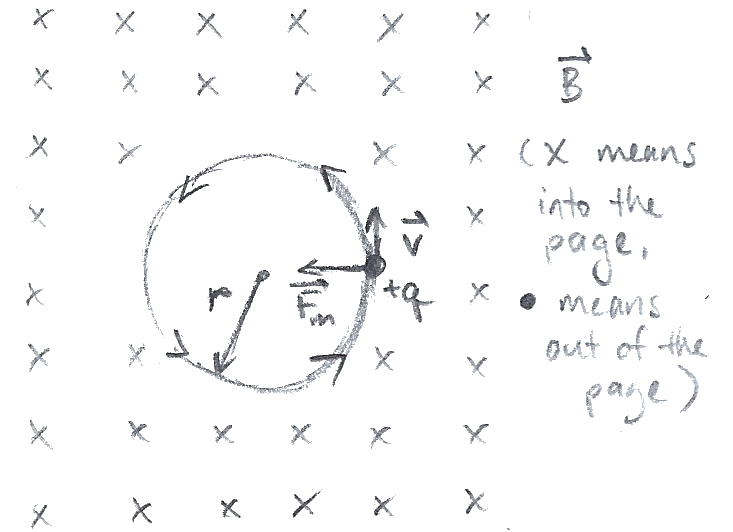
\includegraphics[scale=0.25]{images/em/magnetic-circles.png}
\end{center}
We can find the radius of the motion based on our givens. Using Newton's Second Law (and that the acceleration of a particle in UCM is $\frac{v^2}{r}$, if $r$ is the radius, then we have that:
\[
	m\frac{v^2}{r} = qvB
\]
This rearranges to 
\[
	r = \frac{mv}{qB}
\]
It turns out that the period of this motion is independent of the velocity or radius of the motion. To show this, we can use Newton's Second law to find $\omega = \frac{v}{r}$, which is the angular velocity of the motion:
\[
	\omega = \frac{v}{r} = \frac{q}{m}B
\]
From here, since $T = \frac{2\pi}{\omega}$, we have that 
\[
	T = \frac{2\pi m}{qB}
\]
We can use this to calculate the charge-to-mass ratio of the particle being launched easily since we can control the magnitude of the magnetic field being applied. \\
One last application: what about the magnetic force on a wire due to a current flowing through it? After all, electrons are moving in the wire and can't be dislodged from it, so there is definitely a magnetic force on it. For simplicity, consider a uniform magnetic field $\vec B$, a current $I$ in the wire, and let the wire be straight and have length $L$, have cross-sectional area $A$, and let the number density of electrons per cubic meter be $n$. \\
\begin{center}
	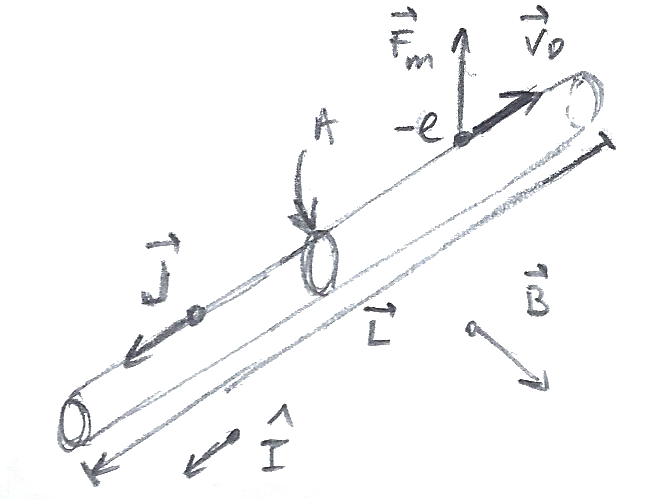
\includegraphics[scale=0.2]{images/em/magnetic-force-wire.png}
\end{center}
On a single charge in the wire drifting along with drift velocity $\vec v_D$, and we can find the magnetic force on each electron (with charge $-e$!):
\[
	\vec F_m = -e\vec v_D \times \vec B
\]
How many electrons are there? It's the volume of the wire times the number density per cubic meter $n$, which is $LAn$. This means the total force $\vec F$ is:
\[
	\vec F = -LAne\vec v_D \times \vec B
\]
We can relate this to the current $I$ - remember that in a conductor we know the current density $\vec j$ is:
\[
	\vec j = -en \vec v_D
\]
Because the charges are negative, they flow OPPOSITE to the current, so $\vec j$ is going in the same direction as the current. We can substitute this in:
\[
	\vec F = AL \vec j \times \vec B
\]
The current and the current density are in the same direction in this straight wire, so let's define a unit vector in that direction $\hat I$. Let's just rewrite this as:
\[
	\vec F = ALj \hat I \times \vec B
\]
Recall that the current $I = jA$ for these uniform wires. Let's have $\vec L = L \hat I$ be the displacement vector along the wire. 
\[
	\vec F = I\vec L \times \vec B
\]
We did this instead of the vector representing the current in the wire because we can actually integrate on the length vectors. For an arbitrary uniform wire, we can look at the differential force $d\vec F$ on the wire by the magnetic field:
\[
	d\vec F = Id\vec l \times \vec B
\]
When we sum up all of these forces:
\[
	\vec F = \sum d\vec F = \sum I d\vec l \times \vec B = I \sum d\vec l \times \vec B
\]
For a current loop, this vector sum becomes zero, because the net displacement around the loop is zero, so the entire product becomes zero. However, there is a torque on this loop. For a small loop of area $A$ and current $I$, define the magnetic moment of the loop to be $\vec \mu = IA\hat n$, where $\hat n$ is the normal unit vector to the plane of the loop. In a uniform magnetic field $\vec B$, it can be shown that the torque on this loop is $\tau = \vec \mu \times \vec B$. This torque tends to line up the magnetic moment with the magnetic field. This motion actually has a potential energy associated with it where $U = -\vec \mu \cdot \vec B$. These are all things that are useful but are just too complicated to prove. \\
There are many other applications for magnetic fields that haven't been discussed, and we'll explore some of them in the problems. 
\subsection{Biot-Savart and Ampere's Laws}
Magnetic fields are induced as a result of the motion of charges - macroscopically, this means currents and its distribution. When we look at magnetic field lines, qualitatively, they form closed loops, unlike that of electric fields due to charges - this can be easily seen by sprinkling a magnetizable material, such as iron shavings, near a magnet. Because the magnetic field lines are closed, it's hard to indicate a direction in which the field lines are going (ie. clockwise or counterclockwise) but we use the right-hand-rule as the arbitrary guideline in this case. For dipoles like magnets, the rule is that the field lines come out from the north pole, loop around the magnet, pass through the south pole and through the body of the magnet to close the loop.\\
\begin{center}
	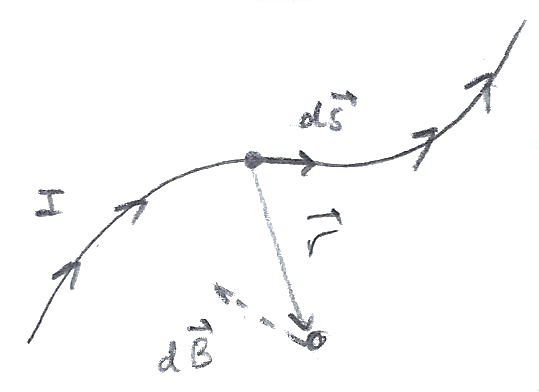
\includegraphics[width=0.4\textwidth]{images/em/biot-savart.png}
\end{center}
Biot and Savart quantitatively derived the magnetic field vector at a point due to a current, and the law used to describe the magnetic field is called (surprise) the Biot-Savart Law. For a uniform length of stationary current that moves $d\vec s$ and $\vec r$ is the displacement vector from the current to the point at which the magnetic field is being calculated, we have that the magnetic field due to this small current is:
\[
	d\vec B = \frac{\mu_0}{4\pi} \frac{I \, d\vec s \times \hat r}{r^2}
\]
where $I$ is the current at that point. The proportionality involves a constant $\mu_0$ that we haven't yet seen - it's called the permeability of free space and has a value of exactly $4 \pi \cdot 10^{-7}$ T$\cdot$m/A. (Alternatively, 1.26 $\cdot$ 10$^{-6}$ T$\cdot$m/A will do just fine.) Similar to Coulomb's Law, Biot-Savart can be used to superpose magnetic fields to calculate the overall magnetic field, and it also follows an inverse-square law similar to that of Coulomb's Law. Therefore, Biot-Savart is useful for calculating the magnetic field due to a complicated configuration of currents, but we can apply it to basically anything - and I'll present the calculations for the field due to an infinite line of current.\\
\begin{center}
    \begin{asy}
        import geometry;
        size(9cm);
        
        real y = 5;
        dot((0, y));

        draw((0,0)--(-10,0), linetype("4 4"), Arrow);
        draw((5.5,0)--(10,0), linetype("4 4"), Arrow);
        draw((-4.25,0)--(0,y), linetype("6 6"));
        draw((0, y)--(0,0));
        draw((-4,0)--(-4.5,0), linewidth(2));
        draw((0,0)--(5.5,0), linetype("4 4"), Arrow);

        label("$y$", (0, y/2), dir(0));
        label("$x$", (-2, -0.5), dir(270));
        label("$dx$", (-4.25, -0.5), dir(270)*0.2);
        label("$I$", (5.5, 0), dir(50));
        label("$P$", (y,0), dir(130));
    \end{asy}
\end{center}
Consider a point $P$ that is a distance $y$ from a uniform line of current carrying a current $I$. Like with the infinite line charge, we can superimpose the real number line on the charge, having the foot of the perpendicular from the point to the line be $x=0$ and extending out to infinity in both directions. Let's arbitrarily have the current running in the $+x$-direction (it won't change the magnitude of the final answer). \\
We know that the magnetic field lines circulate around the current, and the magnitude of the magnetic field due to a small piece of current at a position $x$ going through a displacement $d\vec x$ is:
\[
	d\vec B = \frac{\mu_0}{4\pi} \frac{I \, d\vec x \times \hat r}{x^2+y^2}
\]
Note that all of these small contributions to the field are going to be in the same direction - after all, all of these vectors will be perpendicular to two vectors that lie in the same plane for all values of $x$. We can just consider the magnitude $dB$ because we know the direction by the right-hand rule:
\[
	dB = \frac{\mu_0}{4\pi} \frac{I\, dx}{x^2+y^2} \cdot \frac{y}{\sqrt{x^2+y^2}} =  \frac{\mu_0 Iy\, dx}{4 \pi (x^2+y^2)^{\frac{3}{2}}} 
\]
We integrate with respect to $x$ from $-\infty$ to $\infty$, noting that the integral obtained is very similar to the one we saw before for the infinite line charge (remember we substituted $\theta$ so that $x = y \tan \theta$):
\[
	B = \int_{-\infty}^{\infty} \frac{\mu_0 Iy\, dx}{4 \pi (x^2+y^2)^{\frac{3}{2}}}  = \frac{\mu_0 Iy}{4\pi} \int_{-\infty}^{\infty} \frac{dx}{(x^2+y^2)^{\frac{3}{2}}} = \frac{\mu_0 Iy}{4\pi} \int_{-\frac{\pi}{2}}^{\frac{\pi}{2}} \frac{\cos \theta \, d\theta}{y^2} = \frac{\mu_0 I}{2\pi y} 
\]
This process is non-trivial, but only for a few cases will you have to be able to actually evaluate the integral involved for the magnetic field. \\
Another tool we have for finding the magnetic field (in symmetric cases) is Ampere's Law, which states that the line integral of the magnetic field around a closed loop is directly proportional to the current $I$ passing through the loop:
\[
	\oint_C \vec B \cdot d\vec s = \mu_0 I = \mu_0 \int_S \vec j \cdot \hat n \, dA
\]
Sometimes people will write the current using the third expression using the current density $\vec j$ because it's technically more general, but it's the same. When we calculate this loop integral, we take the normal for the current density integral in agreement with the right-hand rule - that is, whatever direction we integrate around the loop, if your right hand curls around in that direction, the normal should be in the direction of your thumb. The loop used for integrating is often called in Amperian loop (because it's Ampere's Law). It turns out the infinite line of current is basically killed really quickly by this law, which we will see now:\\
\begin{center}
	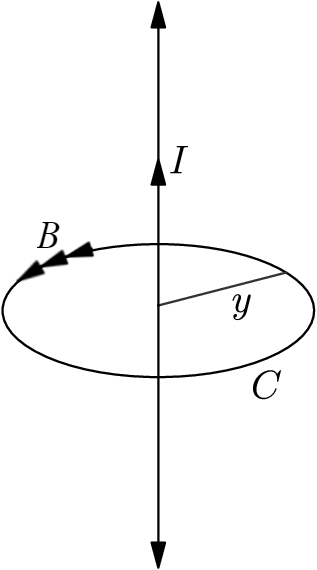
\includegraphics[scale=0.25]{images/em/ampere.png}
\end{center}
Consider the Amperian loop that is a circle centered on the current with radius $y$ passing through the point at which we were calculating the magnetic field. The current through the loop is clearly $I$ because no other currents are in the setup. Usually, we do line integrals around the loop following the right-hand rule (ie. counterclockwise) so since the magnetic field and each displacement around the loop are going in the same direction, the line integral basically evaluates to the circumference times the magnetic field's magnitude. If we substitute into Ampere's Law, we have:
\[
	B \cdot 2\pi y = \mu_0 I
\]
And we can see pretty clearly that we have: 
\[
	B = \frac{\mu_0I}{2\pi y}
\]
just as before. \\
There exist uniform magnetic fields that we haven't explored - the most common one is the field of a solenoid, which is basically a really long coil of wire. We can characterize a solenoid by the number of turns or loops it has, $N$; its length, $L$; and the current through the wire, $I$. 
\begin{center}
	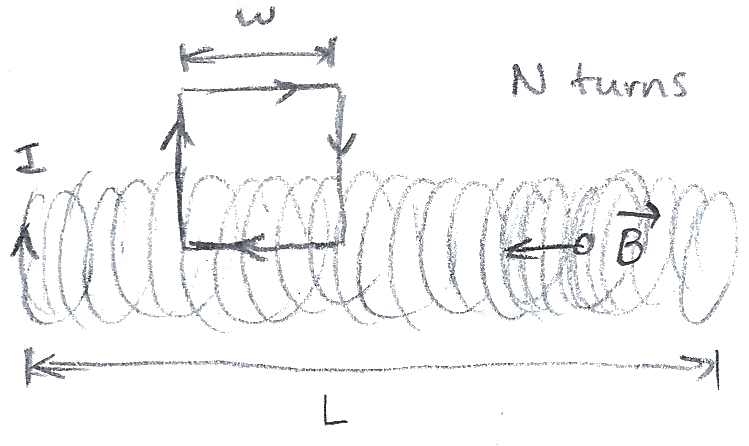
\includegraphics[scale=0.25]{images/em/solenoid.png}
\end{center}
We can use Ampere's Law on a rectangular loop passing through the sides of the solenoid. If the rectangle has width $w$, we can figure out the current passing through the loop:
\[
	\oint_C \vec B \cdot d\vec s = \mu_0 I \frac{N}{L} w
\]
When we integrate around the loop, by symmetry, we know the magnitude of the magnetic field a distance $r$ from the axis of symmetry is all the same. It's also true that the two sides passing through the solenoid will cancel each other out since they're going in different directions. Also, outside of the solenoid, the magnitude of the field is so small that it is effectively zero, especially if the solenoid is really long. Therefore, once we actually evaluate the line integral, we have:
\[
	B(r) w =  \mu_0 I \frac{N}{L} w \quad
	B(r) = \mu_0 I \frac{N}{L}
\]
You might be wondering why we don't have something like Gauss' Law for Magnetism that we can use to calculate magnetic fields. This is because - well, it's not very useful. Similar to electric flux, Gauss' Law uses magnetic flux, which will be discussed at length in the next section - but you can imagine it's similar to electric flux. Gauss' Law for Magnetism states that:
\[
	\oint_S \vec B \cdot \hat n \, dA = 0
\]
This is an interesting result - and we can see that it is true because magnetic field lines form closed loops in space. Because of this, all the field lines must enter and exit the Gaussian surface, so the flux out perfectly cancels the flux in. This means that it's impossible to have some kind of source or sink of the magnetic field - ie. there's no such thing as a magnetic "charge", or monopole, the same way that there is an electric charge (or if there is, we haven't observed it yet). However, it's not terribly useful in calculating the magnetic fields of objects, but it's still important as it implies the non-existence of spherically symmetric magnetic fields. This drastically limits the amount of easily-computable magnetic fields that there are. 
\subsection{Faraday-Lenz's Law and Induction}
We're now going to talk about one of the weirdest things about electricity and magnetism - the concept of induction. First, we have to look at magnetic flux - it's the same thing as electric flux, except for magnetic fields through an area. You can calculate the flux through a flat surface by taking the dot product of the field and the normal vector times the area, and you can break up a curved or weird surface in general into small, infinitesimally small approximately flat surfaces and add up the magnetic flux to find the total:
\[
	\Phi_B = \vec B \cdot \hat n \, A \quad \Phi_B = \int_S \vec B \cdot \hat n \, dA
\] 
It turns out people have a special name for the unit of magnetic flux - it's called a weber (Wb), or a T$\cdot$m$^2$. \\
The magnetic field can be used to generate, or induce, an electric field in a region of space. The Faraday-Lenz Law states that if the magnetic flux is changing with time through some surface bounded by the loop, then an emf is induced in the loop. The rate of change of the magnetic flux is the negative of the emf:
\[
	\oint_C \vec E \cdot d\vec s = \mathscr{E} = -\dv{\Phi_B}{t} = -\dv{}{t} \int_S \vec B \cdot \hat n \, dA
\]
This process is called induction, and in fact, this changing magnetic field generates an electric field that produces this emf. However, the electric field lines here are closed loops and are not like the Coulomb electric fields generated from electric charges and they're non-conservative. \\
Faraday's Law (just the part formulated by Faraday) basically states the magnitude of the emf is equal to the magnitude of the change in the magnetic flux per unit time. However, it's sometimes confusing to figure out which way the emf is going around the loop. Lenz's Law tells us exactly how it's directed - the minus sign in front of the emf indicates that the emf generated opposes the magnetic flux. To be clear, the emf creates a current in the loop, which we know creates its own magnetic field; and Lenz's Law says that this generated magnetic field will try to compensate for the change in the flux and try to stop the change. \\
\begin{center}
	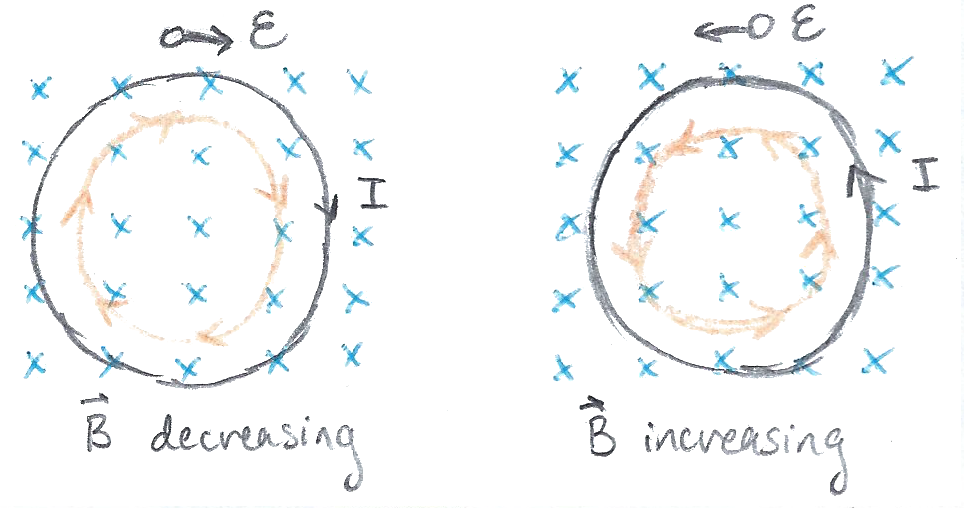
\includegraphics[scale=0.25]{images/em/faraday-lenz.png}
\end{center}
Let's just look at an example. Suppose we have a small circular loop and a magnetic field going into the page and assume the magnitude of the magnetic field is decreasing.\\
Since the magnetic field is decreasing, the emf induced should generate a magnetic field that should increase the magnetic flux. The current around a loop creates a magnetic field according to the right-hand rule - if the fingers curl around in the direction of the current, then the thumb will point in the direction of the magnetic field generated. This means then the magnetic field generated should also point into the page, so the current and emf are directed clockwise around the loop. Similarly, if the magnetic field was increasing, the emf induced should decrease the magnetic flux, which would be achieved if the emf were directed counterclockwise. \\
One of the most common applications of Faraday-Lenz is to a rail gun. Let's consider a metal bar of length $L$ and resistance $R$ sitting on parallel conducting tracks, and the bar can slide back and forth perpendicular to the tracks. There's a battery with emf $\mathscr E$ hooked up to the rails, and a uniform magnetic field $\vec B$ (directed into the page) is present throughout the entire system. Suddenly, the bar is pushed to the right at a velocity $v_0$... and what happens?\\
\begin{center}
	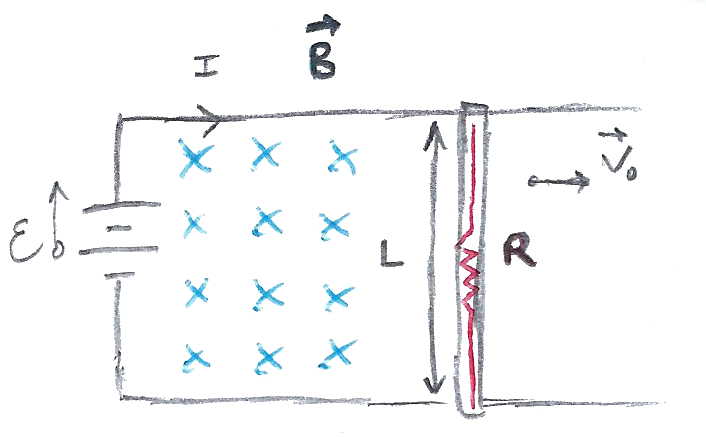
\includegraphics[scale=0.25]{images/em/railgun.png}
\end{center}
Well, let's first just look at the forces on the bar. We could naively say that the force is simply the force on a current that we calculated earlier:
\[
	\vec F = I \vec L \times \vec B 
\]
We know the current is flowing clockwise, so $\vec L$ is directed directly downward, so the resultant force is directed to the right (due to the cross product). This force does non-zero work on the bar because the bar and the force are in the same direction - but this contradicts the fact that forces due to magnetism do not do any work at all! Something is wrong, and it has to do with this analysis of the situation. This formula is only valid if the bar is static and not moving - but once the bar starts to move, other forces are at play. 
The electrons in the bar are both moving rightward with the bar, but also, because of the current, they are also drifting along up the page (as they move opposite to the current due to their negative charge). By the Lorentz Force Law, we can start from scratch and calculate on each electron:
\begin{align*}
	\vec F &= -e(\vec v_D + \vec v_0) \times \vec B\\
	&= -e\vec v_D \times \vec B + (-e) \vec v_0 \times \vec B
\end{align*}
Let's look at these two parts of the term. The first term $-e \vec v_D \times \vec B$ we can recognize as pointing to the right, and from scaling this up by multiplying through by the volume and the density of the electrons, it results in the familiar $I \vec L \times B$ that we know, which does positive work on the bar. \\
On the other hand, the other term $-e \vec v_0 \times \vec B$ is directed down the page, and it pushes all the electrons down the bar. We can see that negative work is done by this force as this magnetic force is exerted on all the electrons traveling down the bar of length $L$. Therefore, the work due to this force is:
\[
	W = -ev_0BL
\]
And as we noted before, the sign is expected to be negative because it needs to cancel the positive work done by the other component of the force. Let's just go one step further and look at the work done per unit charge:
\[
	\mathscr{E}_{ind} = v_0BL
\]
Since we noted that work done by the magnetic force on the electrons in the bar was negative, the work per unit (negative) charge is positive. This work per unit charge is going up the bar, against that exerted by the battery, because negative work is done down the bar. It turns out that this work per unit charge is the induced electromotive force as a result of the changing magnetic flux through the loop formed by the circuit. At least we can see the dimensions are correct through dimensional analysis, but it's not easy to see that this is true. Let's apply Faraday's Law to this situation to see that this is in fact true. \\
In this case, the magnetic flux is increasing not because the field is growing stronger, but because the area is increasing. The area is increasing at a rate of $Lv_0$, so then the rate at which the magnetic flux is changing is:
\[
	\dv{\Phi_B}{t} = BLv_0
\]
The two expressions match in magnitude, but we need to check that the directions of these emfs match. Using Lenz's Law, because the magnetic flux is increasing (and going into the page), the induced emf should create a current that creates a magnetic field going out of the page. This would mean that the current should flow counterclockwise, and so the emf should go counterclockwise, which is consistent with our analysis of the situation using forces. \\
Notice that there's really nothing special about looking at the scenario at $t=0$ - this fact wasn't really ever used, so in general, the emf induced is equal to 
\[
	\mathscr{E} = BLv
\]
where $v$ is the velocity of the bar in the rightward direction at any time. \\
As problems to be solved later, we will look at the current in the bar as a function of time, and the velocity of the bar as a function of time (and note that while the bar shoots off to infinity, it actually eventually reaches a terminal velocity). 
\subsection{Inductance and Circuits Revisited}
With our knowledge of magnetism, we can introduce one last circuit element - the inductor. We have to talk about inductance first, which is a measure of the tendency of a circuit or a conductor (with a closed loop) to induce an emf due to changing currents and has the SI unit of henries (H). Because conductors generate magnetic fields, which are created using current, a changing current will create a changing magnetic field, and therefore a changing magnetic flux. From Faraday-Lenz, we know that a changing magnetic flux in a closed loop will induce an emf in that loop that will act against the change of the magnetic flux. This ratio of the induced emf $\mathscr{E}_{ind}$ to the change in the current per unit time is the inductance $L$, or in other terms:
\[
	\mathscr{E}_{ind} = -L\dv{I}{t}
\]
We can also express the inductance as the ratio of the magnetic flux through a conductor (for loops and coils) to the current through it:
\[
	\Phi_B = LI
\]
This means that 1 H = 1 Wb/A. Furthermore, since the first equation is effectively the time derivative of the second (and an application of Faraday-Lenz) because the derivative of the inductance did not appear, it implies that the inductance $L$ is independent of time. This is true - it turns out the inductance of a conductor is only dependent on the geometry of the conductor, kind of like capacitance is also dependent only on geometry. We can show this is true because the magnetic field is directly proportional to the current, which is also directly proportional to the magnetic flux. \\
Technically speaking, there are two types of inductance - self-inductance and mutual inductance. Self-inductance $L$ is the tendency for a conductor to induce an emf in itself, but mutual inductance $M$ refers to inducing an emf in another conductor (and obeys the same formulas as self-inductance). Most of the time, we will neglect considering the mutual inductance from a conductor to another conductor, because if the current in the first is varying non-linearly, the emf and current produced by the second will create a changing magnetic flux in the first, and soon you have this Russian-nesting-doll type scenario that gets complicated. \\
\begin{center}
	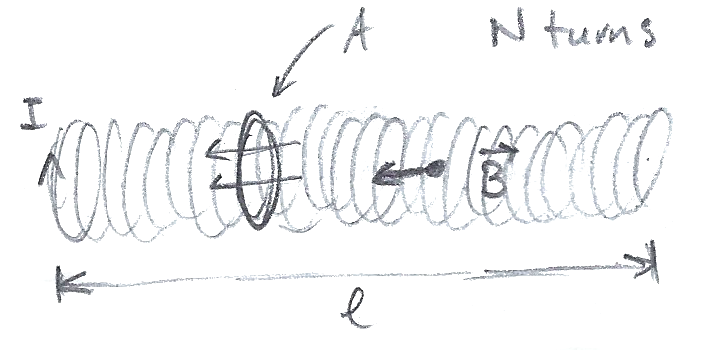
\includegraphics[scale=0.25]{images/em/inductor.png}
\end{center}
As an example, we can look at the self-inductance of a solenoid of $N$ turns with length $l$, cross-sectional area $A$, and current $I$. Remember that the magnetic field of a solenoid is uniform and is:
\[
	B = \mu_0 \frac{N}{l}I
\]
The flux through one turn of the solenoid is the magnetic field times the cross sectional area. However, we have to add up the flux for all the turns, so we have:
\[
	\Phi_B = \mu_0 \frac{N^2A}{l} I
\]
Therefore, the self-inductance $L$ is
\[
	L = \mu_0 \frac{N^2A}{l}
\]
Inductors are circuit elements that have non-negligible self-inductance and as stated earlier, create a resistant emf of magnitude $L\dv{I}{t}$. Work must be done on the inductor in order to get the desired current to flow through the inductor. If we multiply through by the current, we get the rate at which work is done. For a time interval $dt$, the work done on the inductor is then:
\[
	dW = L\dv{I}{t} \cdot I \, dt = LI\, dI
\]
If we increase the current from $0$ to $I$, the work done at the end of the process will be: 
\[
	W = \int_0^I LI\, dI = \frac{1}{2}LI^2
\]
This energy is actually stored in the magnetic field of the inductor, with density per unit volume
\[
	u_B = \frac{1}{2} \frac{B^2}{\mu_0}
\]
As for the case with electric fields, it's difficult to show this is true in the general case, but we can certainly confirm it for our solenoid example. If we plug in our value of the inductance of a solenoid, we can get the energy stored to be:
\[
	U \mu_0 \frac{N^2AI^2}{2l}
\]
The density per unit volume is:
\[
	u_B = \frac{1}{2} \left( \mu_0 \frac{N}{l}I\right)^2 \frac{1}{\mu_0} = \frac{\mu_0 N^2 I^2}{2l^2}
\]
If we multiply through by the volume $Al$, we do get the stored energy in the solenoid, which confirms this formula for this case.\\
In circuits, inductors follow the same rules as resistors because of their similar dependency on the current of the circuit. For two inductors in series with inductances $L_1$ and $L_2$, we have that their effective inductance is 
\[
	L = L_1 + L_2
\]
For the same two inductors in parallel, we have that their effective inductance $L$ is related to these inductances by
\[
	\frac{1}{L} = \frac{1}{L_1} + \frac{1}{L_2}
\]
Again, this is generalizable to larger numbers of inductors. Using these formulas, we can now treat any number of inductors in series or in parallel as essentially one inductor. \\
We are now going to revisit circuitry for real and look at circuits in conjunction with resistors and capacitors. First, let's look at a single-loop LR circuit, with a battery, inductor and a resistor.
\begin{center}
	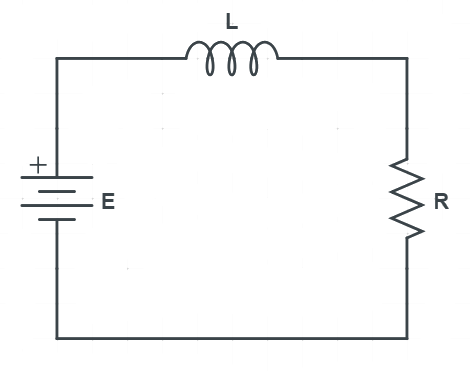
\includegraphics[scale=0.25]{images/em/LR-circuit.png}
\end{center}
Letting the battery have emf $\mathscr{E}$, the resistor a resistance $R$, and the inductor an inductance $L$, we use Kirchhoff's Voltage Law:
\[
	\mathscr{E} - IR - L\dv{I}{t} = 0
\]
We can now rearrange and integrate from time $t=0$ to arbitrary time $t$ just like we did before with an RC circuit, assuming the current at time $t=0$ is zero:\\
\[
	L\dv{I}{t} = \mathscr{E} - IR
\]
\[
	\frac{L}{\mathscr{E} - IR} \dv{I}{t}  = 1
\]
\[
	\int_0^t \frac{L}{\mathscr{E} - IR} \dv{I}{t} \, dt =  \int_0^t 1 \, dt
\]
\[
	-\frac{L}{R} \ln\left(\frac{\mathscr{E} - I(t)R}{\mathscr{E}}\right) = t
\]
\[
	\mathscr{E} - I(t)R = \mathscr{E}e^{-\frac{R}{L}t}
\]
\[
	I(t) = \frac{\mathscr{E}}{R}(1 - e^{-\frac{R}{L}t})
\]
A few remarks: at time $t=0$ the current is $\frac{\mathscr{E}}{R}$, and the inductor doesn't influence the current, so it behaves like a normal wire. However, as $t \to \infty$, the current approaches $0$. This is because inductors take the energy out of the circuit and stores it inside its magnetic field, just like capacitors. However, the increasing magnetic field in the inductor creates an emf against the emf from the battery and eventually stops the flow of current through the inductor, acting like a broken wire. This behavior is general for all inductors. Similar to RC circuits, LR circuits have a time constant $\tau = \frac{L}{R}$, also measuring the speed at which energy is stored into the inductor. From here, we can see that a henry per ohm is also a second - which is a weird combination of units to equal a second, but it works and you can check if you call BS. \\
Moving on to LC circuits - usually, we're only going to consider the starting state to be a fully charged capacitor with capacitance $C$, and an inductor with no current through it with inductance $L$. (You'll see why we've omitted the battery on purpose in this case.) 
\begin{center}
	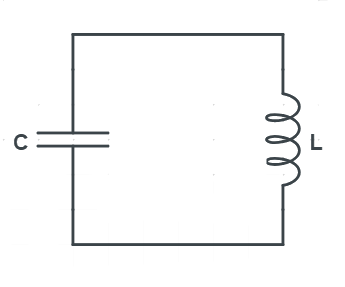
\includegraphics[scale=0.25]{images/em/LC-circuit.png}
\end{center}
Since the capacitor is discharging, it provides a positive emf, while the inductor takes out energy and stores it in its magnetic field. We can use Kirchhoff's Voltage Law:
\[
	\frac{Q}{C} - L \dv{I}{t} = 0
\]
If we note that in this case $I = -\dv{Q}{t}$ (since the charge on the capacitor is decreasing, and the current is always positive) we can rearrange to obtain:
\[
	\frac{Q}{LC} = \dv{I}{t} = -\dv{}{t} \dv{Q}{t} = -\ddv{Q}{t}
\]
This means the second time-derivative of charge is proportional to the charge - which is precisely the differential equation for a simple harmonic oscillator! In this case, the resonant frequency of the circuit is $\omega = \frac{1}{\sqrt{LC}}$. This means that if we consider the charge at time $t=0$ to be $Q_0 > 0$, we can express the charge on the capacitor plates as a function of time to be
\[
	Q(t) = Q_0\cos\left(\frac{1}{\sqrt{LC}}t\right)
\]
where negative values of charge indicate the negative and positive plates of the capacitor have been flipped. Once we take the derivative, we get the current in the circuit at any time to be:
\[
	I(t) = -\frac{Q_0}{\sqrt{LC}}\sin\left(\frac{1}{\sqrt{LC}}t\right)
\]
where negative values of the current indicate the current has changed direction. Because there is no resistance in the circuit, we can see that the stored energy in the circuit is conserved at any given point. Recall that the stored energy in a capacitor is $\frac{1}{2}\frac{Q^2}{C}$, so at the beginning the energy stored is:
\[
	E_{0} = \frac{1}{2}\frac{Q_0^2}{C}
\]
At any given time $t$ the stored energy in the capacitor is:
\[
	E_C = \frac{1}{2}\frac{Q(t)^2}{C} = \frac{1}{2}\frac{Q_0^2 \cos^2\left(\frac{1}{\sqrt{LC}}t\right)}{C}
\]
In the inductor, we can find the energy in the inductor to be:
\[
	E_L = \frac{1}{2}LI^2 = \frac{1}{2}L\left(-\frac{Q_0}{\sqrt{LC}}\sin\left(\frac{1}{\sqrt{LC}}t\right) \right)^2
\]
We can sum this up to find the total energy in the system:
\begin{align*}
	E^{tot} &= \frac{1}{2}\frac{Q_0^2 \cos^2\left(\frac{1}{\sqrt{LC}}t\right)}{C} + \frac{1}{2}L\left(-\frac{Q_0}{\sqrt{LC}}\sin\left(\frac{1}{\sqrt{LC}}t\right) \right)^2 \\
	&= \frac{Q_0^2 \cos^2\left(\frac{1}{\sqrt{LC}}t\right)}{2C} + L\frac{Q_0^2\sin^2\left(\frac{1}{\sqrt{LC}}t\right)}{2LC}\\
	&= \frac{Q_0^2}{2C}\left( \cos^2\left(\frac{1}{\sqrt{LC}}t\right) + \sin^2\left(\frac{1}{\sqrt{LC}}t\right)\right) \\
	&= \frac{Q_0^2}{2C}
\end{align*}
Our results agree, as expected. The time constant for the $LC$ circuit, that is, $\tau = \sqrt{LC}$, shows up everywhere in these calculations, especially because it shows up as the frequency of the circuit. This means the period of the circuit is $T = \frac{2\pi}{\omega} = 2\pi \sqrt{LC}$. (Also, we get one last interesting combination for time - an ohm-henry is a second squared.)\\
Inductors are an important part of circuits that you should know how to handle, and while in general all circuits have inductance, capacitance, and resistance to some degree that you should know how to handle, circuits with all of these explicit elements in them aren't important to AP Physics (because the model for these equations is pretty difficult, but in short, the function for current models dampened oscillations, and looks like a sine wave except as $t \to \infty$ the current goes to zero). Circuits are a difficult concept to master, and it takes a lot of practice and intuition to be able to quickly build the correct quantitative model of the situation.
\subsection{Summary and Problems}
Magnetism is an extremely broad topic - we first looked at how magnetic fields are generated from moving currents and how they exert a force on electric charges. We then looked at magnetic induction and Faraday's Law, where a changing magnetic flux induced an electric field and emf in a loop. Finally, we looked a bit more into the inductance of loops and inductors, the final circuit element involving a magnetic field's effect on creating a voltage drop in the circuit. \\

\noindent \textbf{Problems:}\\
1. (1 $\bigstar$, $\spadesuit$) A current-carrying wire is bent into a closed semicircular loop of radius R that lies in the $xy$-plane. The wire is in a uniform magnetic field that is in the $+z$-direction. Verify that the force acting on the loop is zero. \\
2. (3 $\bigstar$) A simple gaussmeter for measuring horizontal magnetic fields consists of a stiff wire of length $L$ that hangs from a conducting pivot so that its free end makes contact with a pool of mercury in a dish below. The mercury provides an electrical contact without constraining the movement of the wire. The wire has a mass of $m$ and conducts a current downward. If the horizontal magnetic field is $B$ and the current is $I$, show that the equilibrium angular displacement of the wire from vertical is $\theta = \arcsin  \left(\frac{ILB}{mg}\right)$.\\
3. (3 $\bigstar$) A uniform magnetic field $B$ is perpendicular to the base of a hemisphere of radius $R$. Show that the magnetic flux (in terms of $B$ and $R$) through the spherical surface of the hemisphere is $\pi R^2 B$. \\
4. (2 $\bigstar$) A beam of particles with velocity $\vec v$ enters a region that has a uniform magnetic field $\vec B$ in the $+x$-direction. Show that when the velocity of the particle is again in the same direction as it was when the particle entered the field, the $x$-component of the displacement of one of the particles is $\frac{2\pi m}{qB}v \cos \theta$ where $\theta$ is the angle between $\vec v$ and $\vec B$.\\
5. (3 $\bigstar$, $\spadesuit$) Revisit the railgun setup. Consider a metal bar of mass $m$, length $L$, and resistance $R$ sitting on parallel conducting tracks, and the bar can slide back and forth perpendicular to the tracks. A battery with emf $\mathscr E$ is hooked up to the rails, and a uniform magnetic field $\vec B$ goes through the entire region perpendicular to the plane of the tracks. a) If the bar starts from rest, show that the terminal velocity of the bar is $\frac{\mathscr{E}}{BL}$ and that the velocity of the bar as a function of time is $v(t) = \frac{\mathscr{E}}{BL}(1 - e^{-\frac{B^2L^2}{mR}t})$. b) Show that the current in the bar starts at $I = \frac{\mathscr{E}}{R}$, and the current in the bar can be modeled as $I(t) = \frac{\mathscr{E}}{R}e^{-\frac{B^2L^2}{mR}t}$.\\
6. (3 $\bigstar$, $\spadesuit$) Consider a point $P$ on the perpendicular bisector of a wire segment of length $2a$ carrying a current $I$, a distance $R$ away from the midpoint of the segment. a) Show that the magnetic field strength at $P$ is $B = \frac{\mu_0Ia}{2\pi R\sqrt{a^2 + R^2}}$ b) Use your result from part a) to show that the magnetic field strength at the center of a regular polygon of N sides is $\frac{\mu_0IN}{2\pi R} \sin \left(\frac{\pi}{N}\right)$. c) Show that when $N$ is very large, your result approaches that for the magnetic field strength at the center of a circle.\\
7. (2 $\bigstar$) A mass spectrometer uses a velocity selector to guarantee that all the ions enter the main chamber with the same speed. A uniform magnetic field with magnitude $B$ covers the region of the velocity selector and the chamber of the mass spectrometer. In this mass spectrometer, ions with charge $+e$ with different masses will move in a semicircle before colliding with the back wall of the chamber. The spectrometer is designed so that if two ions have a mass difference of $\Delta m$, they will hit the back wall separated by a distance $\Delta x$. Show that the magnitude of the electric field in the velocity selector needs to be $E = \frac{eB^2\Delta x}{2\Delta m}$ for this to work. \\
8. (1 $\bigstar$) The Hall experiment showed that the fundamental charges that we observed around us had a negative sign. Consider a box of height $h$, cross-sectional area $A$, and a uniform magnetic field running parallel to the bottom plane of the box $\vec B$. a) Suppose we inject charged particles into the box moving at a velocity $v$. Show that at equilibrium, the potential difference between the top and bottom of the box is $vhB$. b) Suppose that if we measure the potential difference between the top and bottom of the box to be positive. Show that this is the case if the charges are negative, and the opposite is true if the charges are positive. \\
9. (2 $\bigstar$) A long cylindrical shell has an inner radius $a$ and an outer radius $b$ and carries a current $I$ parallel to the central axis. Assume that within the material of the shell the current density is uniformly distributed. Show that the magnitude of the magnetic field is, if $r$ represents the distance from the central axis, that a) $B = 0$ if $r < a$, b) $B = \frac{\mu_0 I}{2\pi r}\frac{r^2 - a^2}{b^2 - a^2}$ if $b > r > a$, c) $B = \frac{\mu_0 I}{2 \pi r}$ if $r > b$.\\
10. (2 $\bigstar$) At some instant in an oscillating LC circuit, $k$\% of the total energy is stored in the magnetic field of the inductor. a) Show that the multiple of the maximum charge $Q_{max}$ that is on the capacitor is $\sqrt{1-\frac{k}{100}}Q_{max}$ b) Show that the multiple of the maximum current $I_{max}$ that is in the inductor is $\frac{\sqrt{k}}{10}I_{max}$.\\
11. (3 $\bigstar$, $\spadesuit$) In the circuit below, the switch is closed to point $A$ at time $t=0$, with zero initial charge on the capacitor. When the switch is closed, the current is $I_0$. The switch is thrown to point $B$ when the current is $\frac{I_0}{3}$. Show that the maximum current in the inductor after the switch was thrown to point $B$ is $\frac{2}{3} \mathscr{E} \sqrt{\frac{C}{L}}$.
\begin{center}
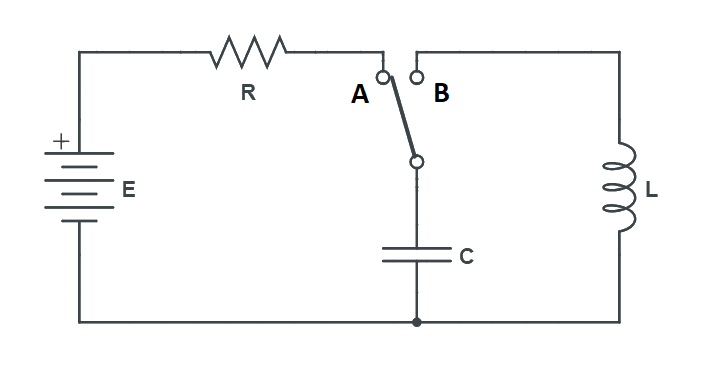
\includegraphics[scale=0.42]{images/em/switchingcircuit.png}
\end{center}
12. (4 $\bigstar$, $\spadesuit$) In the circuit above, the switch is closed to point $A$ at time $t=0$, with zero initial charge on the capacitor. The switch is thrown to point $B$ after a time $\Delta t$. When the energies in the capacitor and in the inductor are equal, show that the current in the inductor is $\mathscr{E}(1- e^{-\frac{t}{RC}})\sqrt{\frac{C}{2L}}$. \\
13. (4 $\bigstar$, $\spadesuit$) A rectangular loop of wire that has width $w$, length $l$, and lies in the vertical plane which is perpendicular to a region that has a uniform magnetic field. The magnitude of the uniform magnetic field is $B$ and the direction of the magnetic field is into the page. The portion of the loop not in the magnetic field has length $y$. The resistance of the loop is $R$ and its mass is
$m$. The loop is released from rest at $t = 0$. (Let down be the $+y$-direction.) Show that the speed of the loop $v$ as a function of time is $v(t) = \frac{mgR}{B^2w^2}(1- e^{-\frac{B^2w^2}{mR}t})$.\\
14. (3 $\bigstar$) A conducting rod of length $l$ rotates at constant angular speed $\omega$ about one end, in a plane perpendicular to a uniform magnetic field $B$. Compute the flux $\Phi_m$ through the area swept out during a time $\Delta t$, and show that the motional emf in the rod is given by $\frac{1}{2}\omega Bl^2$.

\pagebreak